\section{评\ 估}\label{sec:evaluation}

\paragraph{实验环境}

我们在一台拥有Intel E3-1280 V6 CPU、64GB内存、支持SGX v1的服务器上运行程序和进行实验。该机器运行Ubuntu 22.04操作系统,内核版本为5.15.0-56-generic。

\subsection{性能表现}

在这部分,由于其他相关工作都没有开源实现,因此我们只是简单比较了微服务示例程序在SGX内外的通信和计算性能表现。我们将微服务示例程序分别在SGX外的Linux系统和SGX内的运行时内运行,对于每种尺寸的图片测试10次通信和计算开销,并计算得到平均值;在SGX外运行的程序我们使用TLS协议提供通信安全支持。

如图\ref{fig:evaluation}所示,我们可以看到,随着图片尺寸的增大,在SGX内外运行的微服务程序通信延迟都相应增大,在SGX中运行的微服务节点间的通信带来了额外的31.9\%的延迟,推测是数据进出SGX飞地时加解密造成的;但相比于SGX提供的安全保障,这些延迟是可以接受的。而在计算性能方面,SGX内外的计算耗时相比于通信延迟都是可以忽略不计的。

% TODO:重新画图,纵坐标转指数坐标,线性更容易看。

\begin{figure}[!ht]
    \centering
    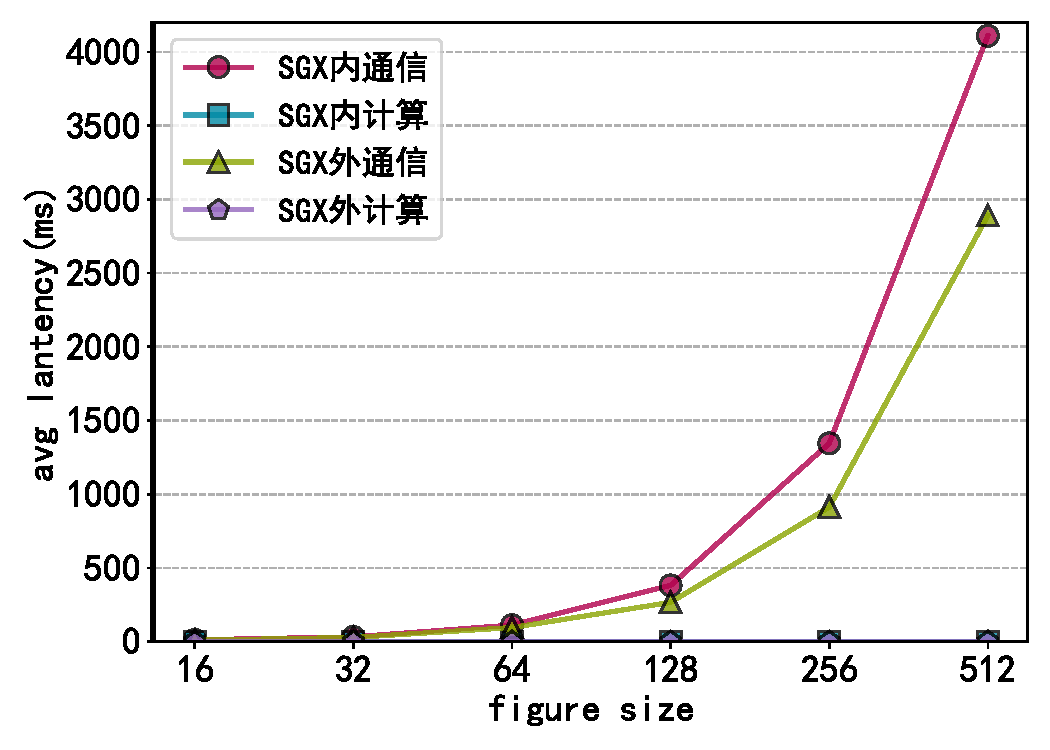
\includegraphics[width=.5\textwidth]{figures/evaluation.pdf}
    \caption{SGX内外微服务通信和计算耗时}
    \label{fig:evaluation}
\end{figure}

\subsection{安全分析}

如~\cref{subsec:threat-model}讲述的威胁模型所示,本次研究主要针对的攻击手段包括系统特权态攻击、网络攻击、漏洞利用攻击等攻击手段,重点防御隐私泄露问题,结合信任模型,我们可以得到如下的安全性分析:

\begin{itemize}
    \item \textbf{系统特权态攻击}:因为硬件和SGX是可信的,因此根据SGX的防御模型,即使OS或HyperVisor是恶意的或被劫持,SGX中的数据也不会泄露,因此本平台可以防御系统特权态攻击。
    \item \textbf{中间人攻击}:对于中间人攻击,我们使用了DHKE协议来协商对称共享密钥,用以加密保证通信的安全性;即使所有的DH共享参数都被中间人截获,中间人也无法得到密钥,因此无法解读加密信息。同时通过使用SGX远程验证,可以验证微服务节点身份的真实性,防止中间人伪造节点进行攻击。
    \item \textbf{重放攻击}:对于重放攻击,我们在通信协议中加入了计数器,且借助SGX和微服务计算场景的特点,消除了TLS 0-RTT状态恢复情况的漏洞,可以成功过滤掉重放攻击。
    \item \textbf{内存攻击}:对于系统编程语言容易出现的悬垂指针、缓冲区溢出等漏洞带来的内存攻击,我们选择使用安全编程语言Rust,结合其强大的静态分析能力,基本可以消除这些漏洞(除非使用unsafe)。
    \item \textbf{权限扩散}:我们使用JWT的方法进行授权管理,类似于基于功能(Capability)的思想,为了防止权限扩散到下级节点,我们使用了Token交换的授权管理方法,可以实现细粒度的授权管理,减少隐私扩散。
\end{itemize}

另外,在一个完善的微服务场景中,还可能存在物理攻击、DDoS攻击、针对数据库的攻击等,但是针对这些攻击的应对措施与本次研究是正交的领域,因此不在本次研究的讨论范围内。
